\documentclass{article}

\pagestyle{plain} % removes running headers

\usepackage{booktabs} % For formal tables

\usepackage{hyperref}
%\usepackage[usenames]{color}
\usepackage[usenames, dvipsnames]{color}
\usepackage{epsfig}
\usepackage{bbm}
\usepackage{graphicx}
\usepackage{amsmath, amssymb}
\usepackage[ruled]{algorithm2e}
\usepackage{empheq}
\usepackage{thmtools,thm-restate}
\usepackage{framed}
\let\labelindent\relax
\usepackage{enumitem}
\usepackage{letltxmacro}
\usepackage{subfig}
\usepackage{multirow}
%\usepackage{subfigure}
%\usepackage[table]{xcolor}
\pagenumbering{arabic}
\usepackage[most]{tcolorbox}

%\newdef{Claim}{Claim}
%\newdef{Example}{Example}
\newtheorem{ppt}{Property}
\newtheorem{cor}{Corollary}
\newtheorem{prop}{Proposition}
\newtheorem{lemma}{Lemma}
\newtheorem{thm}{Theorem}

\newcommand\XXXNote[1]{\textcolor{red}{[\bf #1]}}
\newcommand{\red}[1]{\textcolor{red}{#1}}
\newcommand{\blue}[1]{\textcolor{blue}{#1}}
\newcommand{\anote}[1]{\textcolor{magenta}{[\bf AM: #1]}}

\newcommand{\reals}{{\mathbb R}}
\newcommand{\prob}{\mathbb P}
\newcommand{\E}{\mathbb E}
\newcommand{\algo}{dandelion}
\newcommand{\Algo}{{\sc Dandelion}}
\newcommand{\Algopp}{{\sc TwistedPair}}
\DeclareMathOperator*{\argmin}{arg\,min}
\DeclareMathOperator*{\R}{\mathbb R}
\DeclareMathOperator*{\Z}{\mathbb Z}
\DeclareMathOperator*{\dist}{\text{dist}}
\DeclareMathOperator*{\argmax}{arg\,max}
\DeclareMathOperator*{\detec}{\hat v = v}

\usepackage{listings}
%\usepackage{minted}
\usepackage{color} %red, green, blue, yellow, cyan, magenta, black, white
\definecolor{mygreen}{RGB}{28,172,0} % color values Red, Green, Blue
\definecolor{mylilas}{RGB}{170,55,241}

%\newdef{Claim}{Claim}
%\newdef{Example}{Example}

\newcommand{\bb}{\mathbf{b}}
\newcommand{\bx}{\mathbf{x}}
\newcommand{\by}{\mathbf{y}}
\newcommand{\be}{\mathbf{e}}
%\newcommand{\b0}{\mathbf{0}}
\newcommand{\bI}{\mathbf{I}}
\newcommand{\diag}{\text{diag}}
\newcommand{\tr}{\text{tr}}
%\DeclareMathOperator*{\N}{\mathbb N}

\makeatletter
\newcommand{\removelatexerror}{\let\@latex@error\@gobble}
\makeatother

\sloppy


\begin{document}
\title{Homework 2}
\author{Optimization, 18-660/18-460 \\ \textbf{Out:} Feb 10, 2026 \\ \textbf{Due:}  Feb. 27, 2026 by 11:59 pm EST}
\date{}
\maketitle

\section*{Instructions}
\begin{itemize}
	\item \textbf{Collaboration Policy: } See syllabus for collaboration policy.
	      You need to fill out the declaration page at the end of this PDF and append it to your homework submission.
	      \textbf{\emph{Failure to submit the declaration page will lead to a panelty on assignment credit.}}
	\item \textbf{Submission Instructions: } Assignments should be submitted as pdfs on Gradescope.
	      Each problem should be on a separate page.
	      When submitting to Gradscope, make sure to label each question using the interface provided by Gradescope. If you do not do this, your assignment WILL NOT be graded!
	\item \textbf{Programming: } Programming assignments should also be submitted to Gradescope. If you are not planning to use MATLAB or Python for your submission, please clear your choice with the instructors before submitting.
	\item \textbf{Late Policy: } You may use up to 3 late days on a single assignment. The maximum total number of late days allowed across all assignments is 5.
\end{itemize}

% problem 1
\newpage
\section*{Problem 1: Optimization Problems (30 points)}
\begin{enumerate}
\item \textbf{[10 points]} Prove that for convex optimization, a local minimizer is a global minimizer. More specifically, consider a convex optimization problem $\min_{x\in C} f(x)$, where $C$ is a convex set and $f(x)$ is differentiable. Suppose $x^*$ is a local minimizer, i.e. $\exists \delta>0$ s.t. for all $x \in C\cap B_\delta(x^*)$ (where $B_\delta(x^*) = \{ x:\Vert x-x_*\Vert_2 \leq \delta\}$), $f(x)\geq f(x^*)$. Prove that such an $x^*$ is a global optimizer for the optimization problem, that is $f(x)\geq f(x^*) $ for all $x\in C$. (Hint: show the first order optimality condition holds for $x^*$. You may use contradiction arguments similar to the ones used in lecture 5.)
	    \begin{tcolorbox}
		% Your solution here
	\end{tcolorbox}
\item  \textbf{[10 points]} Consider a symmetric matrix $X \in \mathbb S^n$ (Recall that $\mathbb S^n$ denotes the set of $n\times n$ symmetric matrices.) written in block form:
\begin{equation*}
X = 
\begin{bmatrix}
A & B \\
B^\top  & C
\end{bmatrix}
\end{equation*}
with $A\in \mathbb S^k$ and $A$ nonsingular, $C\in\mathbb{S}^{n-k}$, and $B\in\mathbb{R}^{k\times (n-k)}$. The matrix 
$$
S = C-B^\top  A^{-1}B
$$
is called the Schur complement of $A$ in $X$. 
	\begin{enumerate}
	\item \textbf{[5 points]} Suppose $A\succ 0$, i.e., $A$ is positive definite. Consider the optimization problem
    $$
    \min_{u\in \mathbb{R}^k} u^\top  Au + 2u^\top Bv  + v^\top Cv
    $$
    where $u$ is to be optimized and $v\in \mathbb{R}^{n-k}$ is fixed. Compute the optimal value of this problem as a function of $v$ and $S$.
    \begin{tcolorbox}
		% Your solution here
	\end{tcolorbox}
	\item \textbf{[5 points]} Suppose $A \succ 0$. Prove that $X\succeq 0$ if and only if $S \succeq 0$.  (Hint: note the objective function in part (a) can be written as $\begin{bmatrix} u\\v\end{bmatrix}^\top  X \begin{bmatrix} u\\v\end{bmatrix} $)
	\begin{tcolorbox}
		% Your solution here
	\end{tcolorbox}
	\end{enumerate}


\item \textbf{[10 points]}  \emph{(Optional for 18-460 students)}  Show that SOCPs can be written as SDPs. For simplicity, you may consider the following simplified version of SOCP :
\begin{align*}
	\min_{x\in\mathbb{R}^n} & f^\top  x \\
	\text{ s.t. }  \Vert Ax + b\Vert_2 &\leq c^\top x + d,
\end{align*}
for some $f,c\in\mathbb{R}^n$, $A\in \mathbb{R}^{m\times n}$, $b\in \mathbb{R}^m$, $d\in\mathbb{R}$. 
 Show that the above problem can be written as an SDP. (Hint: try to write the inequality $\Vert Ax + b\Vert_2 \leq c^\top x + d$ as an SDP constraint using Schur Complement in part 2 of the problem. )
\begin{tcolorbox}
		% Your solution here
	\end{tcolorbox}
\end{enumerate}

% problem 2
\newpage
\lstset{language=Matlab,%
    %basicstyle=\color{red},
    breaklines=true,%
    morekeywords={matlab2tikz},
    keywordstyle=\color{blue},%
    morekeywords=[2]{1}, keywordstyle=[2]{\color{black}},
    identifierstyle=\color{black},%
    stringstyle=\color{mylilas},
    commentstyle=\color{mygreen},%
    showstringspaces=false,%without this there will be a symbol in the places where there is a space
    numbers=left,%
    numberstyle={\tiny \color{black}},% size of the numbers
    numbersep=9pt, % this defines how far the numbers are from the text
    emph=[1]{for,end,break},emphstyle=[1]\color{red}, %some words to emphasise
    %emph=[2]{word1,word2}, emphstyle=[2]{style},    
}
\section*{Problem 2: Canonical Forms - Solving different forms of Compressive Sensing with CVX  (30 points)}

Compressive sensing (also known as compressed sensing, compressive sampling, or sparse sampling) is a signal processing technique for efficiently acquiring and reconstructing a signal, by finding solutions to under-determined linear systems. This is based on the principle that, through optimization, the sparsity of a signal can be exploited to recover it from far fewer samples than required by the Shannon-Nyquist sampling theorem. There are two conditions under which recovery is possible. The first one is sparsity which requires the signal to be sparse in some domain. The second one is incoherence which is applied through the isometric property which is sufficient for sparse signals. --- From Wikipedia. 

Compressive sensing is used in single-pixel camera (SPC), which is shown in Fig. \ref{fig:SPC}. In SPC, in addition to the sensor, we add a light modulator, a digital micromirror device (DMD). The scene is first focused on the DMD which in turn is focused on a photo-detector. DMD can display masks to code the scene. The DMD and the photo-detector are synchronized. Every time the DMD codes the scene, the photo-detector obtains sum of the coded scene. By changing the mask on the DMD, the photo-detector obtains different measurements of the scene. After taking enough measurements, we can reconstruct the scene. SPC has broad usage. For example, a traditional 2D short-wave infrared imager costs tens of thousands of dollars while SPC costs less than hundreds of dollars.

Denote $\bx \in \R^n$ as vectorized image (concatenating columns of a 2D image into one column), $A \in \R^{m\times n}$ as measurement matrix where each row corresponds to one mask on the DMD, and $\bb \in \R^m$ as measurements by the photo-detector. We have $$\bb = A\bx + \be$$ where $\be$ is the noise. By compressive sensing, $\bx$ can be reconstructed even if $m \ll n$. We exploit the image prior that image gradient is usually sparse (i.e. $x_i - x_j$ are mostly $0$ when $i$ and $j$ are adjacent pixels in the image) to reconstruct the image in this problem.\\
\begin{figure}[!htb]
\centering
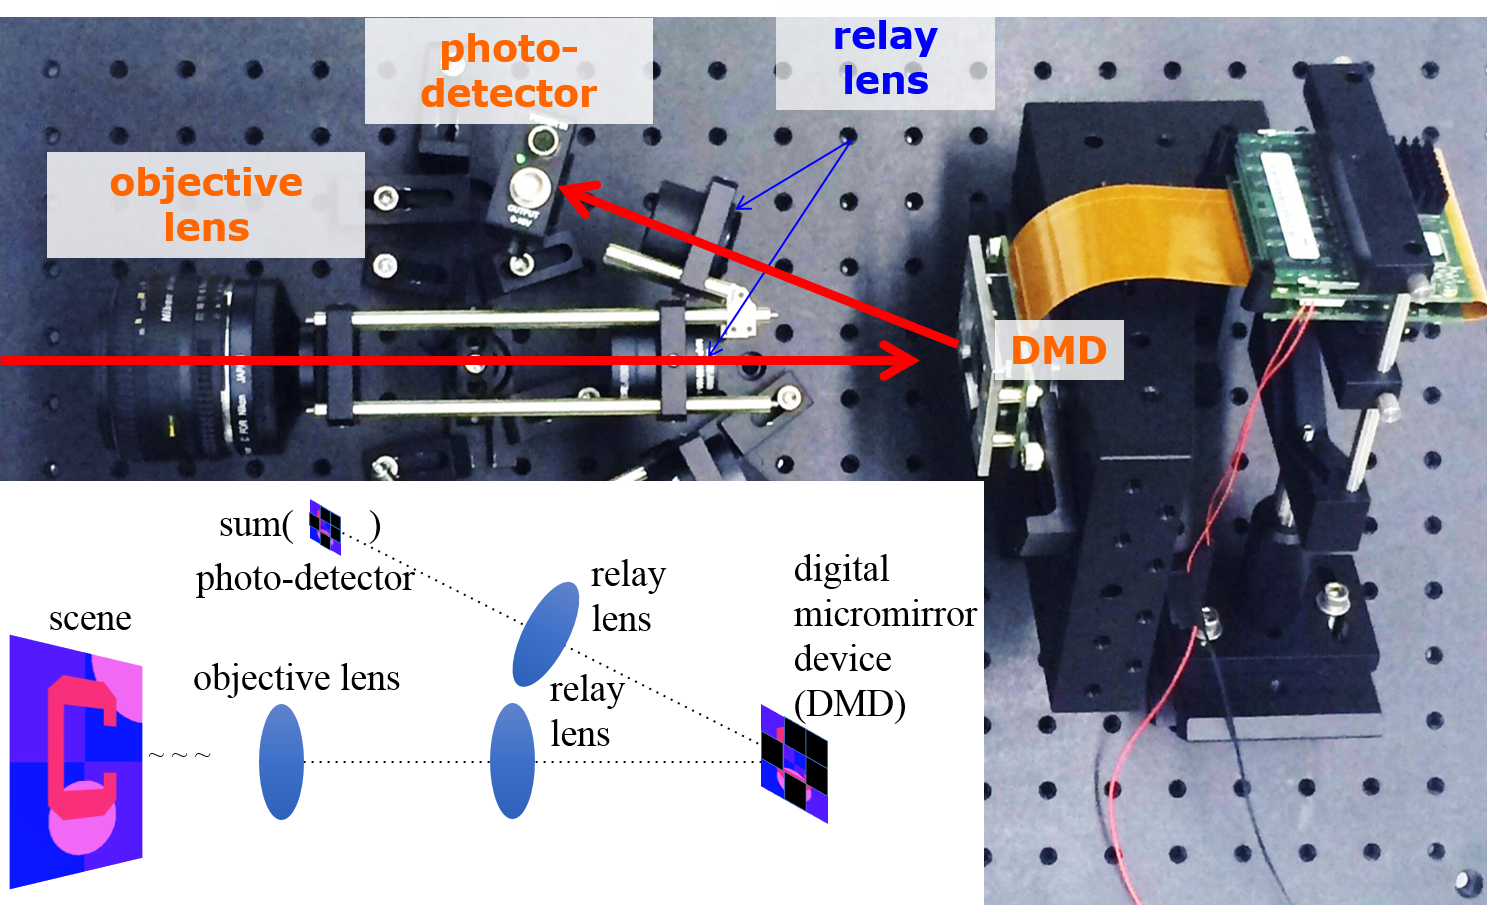
\includegraphics[width=0.75\textwidth]{images/SPC.png} 
\caption{Single pixel camera. }
	\label{fig:SPC}
\end{figure}

\bigskip
\noindent
\begin{enumerate}

\item \textbf{[10 points]} Suppose there is no measurement noise. We will solve this problem:
\begin{equation}\label{}
\begin{split}
&\min_\bx  \; \sum_{\{i,j\} \in E}|x_i - x_{j}|  \\
&\text{ \,s.t.\,\, } A\bx = \bb
\end{split}
\end{equation}
The set $E$ is the set of all undirected edges connecting horizontally or
vertically neighboring pixels in the image. More specifically, $\{i,j\} \in E$
if and only if pixel $i$ is the immediate neighbor of pixel $j$ on the left,
right, above or below. 

	\begin{enumerate}
    	\item Can this problem be transformed to LP, QP or SOCP? Why? (We know that LP $\subset$ QP $\subset$ SOCP, so choose the smallest set that contains this problem; same for next problems.)
	\begin{tcolorbox}
		% Your solution here
	\end{tcolorbox}
        \item Load the measurement matrix $A$ and measurement data $\bb$ from Canvas SPC.mat (scipy.io.loadmat can be used to load the .mat file in Python), and solve $\bx \in \R^{1024}$ which is actually vectorized $32\times 32$ image using CVX ({\it Hint: Image $\bx$ is a matrix that has been vectorized by concatenating its rows. Write the objective function in matrix form}). Show your reconstructed image (for example, in Matlab use imshow() function). \\If measurement ratio is defined as the number of measurements over the number of pixels which is dimension of $\bb$ over dimension of $\bx$ here, note here measurement ratio is $30\%$. 
        \begin{tcolorbox}
		% Your solution here
	\end{tcolorbox}
    \end{enumerate}
    
\item \textbf{[10 points]} When there is measurement noise, we can solve this problem:
\begin{equation}\label{}
\min_\bx  \; \frac{1}{2}\|A\bx-\bb_n \|_2^2 + \lambda \sum_{\{i,j\} \in E}|x_i - x_{j}|  
\end{equation}
where $\bb_n$ are noisy measurements.
The set $E$ is defined same as last problem. 

	\begin{enumerate}
    	\item Can this problem be transformed to LP, QP or SOCP? Why?
	\begin{tcolorbox}
		% Your solution here
	\end{tcolorbox}
        \item Load $A$ and the noisy measurement data $\bb_n$ from Canvas SPC.mat, choose 
        $\lambda \in \{ 0.1, 1, 10, 100\}$ and solve $\bx$ using CVX. Show images with all $\lambda$s.
        \begin{tcolorbox}
		% Your solution here
	\end{tcolorbox}
    \end{enumerate}
    
\item \textbf{[10 points]} When we know the measurement noise $\Vert \mathbf{e}\Vert $ are upper bounded by $\epsilon$, we can solve this problem:
\begin{equation}\label{}
\begin{split}
&\min_\bx  \; \sum_{\{i,j\} \in E}|x_i - x_{j}|  \\
&\text{ \,s.t.\,\, } \| A\bx - \bb_n \|_2 \leq \epsilon
\end{split}
\end{equation}

\begin{enumerate}
    	\item Can this problem be transformed to LP, QP or SOCP? Why? 
	\begin{tcolorbox}
		% Your solution here
	\end{tcolorbox}
        \item Load $A$ and the noisy measurement data $\bb_n$ from Canvas SPC.mat. We know that the measurement noise, which is readout noise here, is i.i.d. with mean 0 and variance 1, i.e. $\be \sim \mathcal{N}(\mathbf{0}, \bI)$.
Choose suitable $\epsilon$ and solve $\bx$ using CVX. Show the image.
\begin{tcolorbox}
		% Your solution here
	\end{tcolorbox}
    \end{enumerate}

\end{enumerate}

% problem 3
\newpage
\section*{Problem 3: Gradient Descent (40 points)}
We have proved that for a convex and $L$-smooth function
$f:\mathbb{R}^n \rightarrow \mathbb{R}$, the
convergence rate for gradient descent is $\mathcal{O}(1/k)$ where $k$ is
the number of iterations.
More precisely, we proved that
\begin{align}
	f(x(k)) - f^* \le \frac{\|x(0) - x^*\|^2_2}{2\alpha k}
\end{align}
where $0 < \alpha \leq 1/L$ is a fixed step size, $L$ is the Lipschitz
constant of the gradient of $f$, $x(0)$ is the starting point, $x(k+1) = x(k) - \alpha \nabla f(x(k))$,
$x^*$ is an optimizer and $f^* = f(x^*)$, and
$k$ is the number of iterations. 

We also mentioned that if $f$ is
also strongly convex with parameter $\mu$, 
then the rate of convergence for gradient descent is $\mathcal{O}(c^k)$.
In this exercise, we will prove this result.\\

\noindent
(a) \textbf{[8 points]} \emph{(Optional for \textbf{all} students)} Suppose a function $g:\mathbb{R}^n\rightarrow \mathbb{R}$ is convex and $L$-smooth. Show that:
\begin{align}
\label{eq:3a}
g(y) \ge g(x) + \nabla g(x)^\top (y-x) + \frac{1}{2L}\|\nabla g(y) - \nabla g(x)\|_2^2.
\end{align}
for any $x, y \in \mathbb{R}^n$.

\noindent
\textbf{Hint:} write down
\begin{align*}
g(x) + \nabla g(x)^\top(z-x) \le g(z) \le g(y) + \nabla g(y)^\top(z-y) + \frac{L}{2}\|z-y\|_2^2
\end{align*}
and let $z$ to take a best value.
\begin{tcolorbox}
		% Your solution here
	\end{tcolorbox}

\noindent\textbf{For part (b)-(e), we assume that $f$ is $\mu$-strongly convex and $L$-smooth. }

\noindent (b) \textbf{[12 points]} \emph{(Optional for 18-460 students)} Use the result of part (a) to show that
\begin{align}
	\left\langle \nabla f(x) - \nabla f(y), x - y \right\rangle \ge
    \frac{\mu L}{\mu+L} \|x - y\|^2_2 + \frac{1}{\mu+L} \|\nabla f(x) - \nabla f(y)\|^2_2
\end{align}
for any $x,y \in \mathbb{R}^n$.

\noindent
\textbf{Hint:} Let $g(x) = f(x) - \frac{\mu}{2}\|x\|_2^2$ and apply (\ref{eq:3a}) on $g$ for both $(x,y)$ and $(y,x)$. 
\begin{tcolorbox}
		% Your solution here
	\end{tcolorbox}

\noindent
(c) \textbf{[12 points]} \emph{(Optional for 18-460 students)} Throughout this exercise, the step size $\alpha$ is assumed to a fixed
number (across the gradient descent iterations) and $0 < \alpha \le 2/(\mu+L)$. Use the result of part (b) to show that
\begin{align}
	\|x(k) - x^*\|^2_2 \le \left(1 - \frac{2\alpha \mu L}{\mu+L} \right)^k \|x(0) - x^*\|^2_2
\end{align}
\textbf{Hint:} Try to show the following descent inequality: $	\|x(k) - x^*\|^2_2 \le \left(1 - \frac{2\alpha \mu L}{\mu+L} \right) \|x(k-1) - x^*\|^2_2$
\begin{tcolorbox}
		% Your solution here
	\end{tcolorbox}

\noindent
(d) \textbf{[10 points]} Use the result of part (c) to prove that
\begin{align}
	f(x(k)) - f^* \le \frac{L}{2} \left( 1 - \frac{2\alpha \mu L}{\mu+L} \right)^k \|x(0) - x^*\|^2_2
\end{align}
\begin{tcolorbox}
		% Your solution here
	\end{tcolorbox}
	
\noindent
(e) \textbf{[6 points]} Show that the optimal rate of convergence is
\begin{align}
	c = \min_{0 < \alpha \le 2/(m+L)} \left( 1 - \frac{2\alpha \mu L}{\mu+L} \right) = \left(\frac{\kappa -1}{\kappa+1}\right)^2
\end{align}
where $\kappa =L/\mu$ is the condition number of $f$. 
\begin{tcolorbox}
		% Your solution here
	\end{tcolorbox}



% ========== THE END ==========
\newpage
\section*{Declaration of External Resources}

Please fill out the following information with handwriting/typing and append this page to your homework submission.
\textbf{\emph{Failure to submit this declaration page will lead to a panelty on assignment credit.}}
You can use extra sheets of paper to answer the following questions if you need more space.

1. Have you collaborated with other students? If yes, name the collaborators and briefly describe the nature of collaboration.

Yes $\square$ \quad No $\square$

\begin{tcolorbox}
	% Your solution here
	\vspace{1in}
\end{tcolorbox}

2. Have you used GenAI in helping solve the problem? If yes, provide a brief description of how you used GenAI. You can also optionally append your chat history to your homework submission.

Yes $\square$ \quad No $\square$

\begin{tcolorbox}
	% Your solution here
	\vspace{1in}
\end{tcolorbox}

3. Cite all other external resources you used to finish the assignment.

\begin{tcolorbox}
	% Your solution here
	\vspace{1.6in}
\end{tcolorbox}

\end{document}